This section assumes that the user passed a set of text documents and 
specified a set of tag types using the interactive user friendly
interface of \framework. 
Let $T=\langle t_1,t_2,\ldots,t_M\rangle$ be a set of Arabic words denoting the 
text documents, and let ${\cal T}$  be the 
set of tag types each with an associated formula. 
\framework uses Sarf~\cite{ZaMaColing2012DemosSarf},
to compute a set of morphological solutions $M(t)=\{m_1,m_2,\ldots,m_N\}$
for each word $t\in T$. 

Recall from Section~\ref{sec:overview} 
that \pp, \ss, \xx, \PP, \GG, and \AC~denote the set of prefixes, stems, 
suffixes, POS, gloss, and category tags, respectively. 
Each morphological solution $m\in M(t)$ is a tuple of the form 
$\langle p,s,x,P,G,C\rangle\in \pp \times  \ss\times \xx\times \PP\times\GG \times \AC$.
%where $p\in \pp, s\in \ss, x\in \xx, P \in \PP, G \in \GG,$ and $C \in \AC$. 

In what follows we formally present 
the extended synonymy feature, 
the morphology-based atomic terms (MAT), 
the morphology-based Boolean formulae (MBF), 
the morphology-based regular expressions (MRE), 
the computational actions, and the user defined relational entities.
 
%\begin{table}[tb!]
%\centering
%\caption{Example of computing $Sy(l_{5})$ and $Sy^{1}(l_{5})$}
%\begin{tabular}{|c|c|c|c|c|c|}
%\hline
%$s$ & $\alpha(s) $ & $\alpha(l_{1})\cap\alpha(s)$ & $\alpha(l_{2})\cap\alpha(s)$ & $\alpha(l_{3})\cap\alpha(s)$ \\
%\hline
%$l_{1}$ & $e_{1}$,$e_{2}$ & $e_{1}$,$e_{2}$ & $e_{2}$ & $e_{2}$ \\
%\hline
%$l_{2}$ & $e_{2}$ & $e_{2}$ & $e_{2}$ & $e_{2}$ \\
%\hline
%$l_{3}$ & $e_{2},e_{3}$ & $e_{2}$ & $e_{2}$ & $e_{2},e_{3}$ \\ 
%\hline
%$l_{4}$ & $e_{3},e_{4}$ & $\emptyset$ & $\emptyset$ & $e_{3}$ \\
%\hline 
%\end{tabular}
%\label{table:syex}
%\end{table}
%

\begin{figure}[tb!]
\setcode{utf8}
\begin{center}
  \resizebox{\columnwidth}{!}{ 
  	{\relsize{-3} % Graphic for TeX using PGF
% Title: /home/ameen/Desktop/Syn.dia
% Creator: Dia v0.97.1
% CreationDate: Fri Mar  7 00:34:04 2014
% For: ameen
% \usepackage{tikz}
% The following commands are not supported in PSTricks at present
% We define them conditionally, so when they are implemented,
% this pgf file will use them.
\ifx\du\undefined
  \newlength{\du}
\fi
\setlength{\du}{15\unitlength}
\begin{tikzpicture}
\pgftransformxscale{1.000000}
\pgftransformyscale{-1.000000}
\definecolor{dialinecolor}{rgb}{0.000000, 0.000000, 0.000000}
\pgfsetstrokecolor{dialinecolor}
\definecolor{dialinecolor}{rgb}{1.000000, 1.000000, 1.000000}
\pgfsetfillcolor{dialinecolor}
\definecolor{dialinecolor}{rgb}{1.000000, 1.000000, 1.000000}
\pgfsetfillcolor{dialinecolor}
\pgfpathellipse{\pgfpoint{3.630147\du}{12.268195\du}}{\pgfpoint{0.803947\du}{0\du}}{\pgfpoint{0\du}{0.833295\du}}
\pgfusepath{fill}
\pgfsetlinewidth{0.020000\du}
\pgfsetdash{{\pgflinewidth}{0.200000\du}}{0cm}
\pgfsetdash{{\pgflinewidth}{0.200000\du}}{0cm}
\pgfsetmiterjoin
\definecolor{dialinecolor}{rgb}{0.000000, 0.000000, 0.000000}
\pgfsetstrokecolor{dialinecolor}
\pgfpathellipse{\pgfpoint{3.630147\du}{12.268195\du}}{\pgfpoint{0.803947\du}{0\du}}{\pgfpoint{0\du}{0.833295\du}}
\pgfusepath{stroke}
% setfont left to latex
\definecolor{dialinecolor}{rgb}{0.000000, 0.000000, 0.000000}
\pgfsetstrokecolor{dialinecolor}
\node at (3.630147\du,12.371528\du){\RL{ماء}};
\definecolor{dialinecolor}{rgb}{1.000000, 1.000000, 1.000000}
\pgfsetfillcolor{dialinecolor}
\pgfpathellipse{\pgfpoint{7.412496\du}{12.443762\du}}{\pgfpoint{0.899916\du}{0\du}}{\pgfpoint{0\du}{0.848262\du}}
\pgfusepath{fill}
\pgfsetlinewidth{0.020000\du}
\pgfsetdash{{\pgflinewidth}{0.200000\du}}{0cm}
\pgfsetdash{{\pgflinewidth}{0.200000\du}}{0cm}
\pgfsetmiterjoin
\definecolor{dialinecolor}{rgb}{0.000000, 0.000000, 0.000000}
\pgfsetstrokecolor{dialinecolor}
\pgfpathellipse{\pgfpoint{7.412496\du}{12.443762\du}}{\pgfpoint{0.899916\du}{0\du}}{\pgfpoint{0\du}{0.848262\du}}
\pgfusepath{stroke}
% setfont left to latex
\definecolor{dialinecolor}{rgb}{0.000000, 0.000000, 0.000000}
\pgfsetstrokecolor{dialinecolor}
\node at (7.412496\du,12.547096\du){\RL{نضح}};
\definecolor{dialinecolor}{rgb}{1.000000, 1.000000, 1.000000}
\pgfsetfillcolor{dialinecolor}
\pgfpathellipse{\pgfpoint{11.327704\du}{12.243392\du}}{\pgfpoint{0.887504\du}{0\du}}{\pgfpoint{0\du}{0.840661\du}}
\pgfusepath{fill}
\pgfsetlinewidth{0.020000\du}
\pgfsetdash{{\pgflinewidth}{0.200000\du}}{0cm}
\pgfsetdash{{\pgflinewidth}{0.200000\du}}{0cm}
\pgfsetmiterjoin
\definecolor{dialinecolor}{rgb}{0.000000, 0.000000, 0.000000}
\pgfsetstrokecolor{dialinecolor}
\pgfpathellipse{\pgfpoint{11.327704\du}{12.243392\du}}{\pgfpoint{0.887504\du}{0\du}}{\pgfpoint{0\du}{0.840661\du}}
\pgfusepath{stroke}
% setfont left to latex
\definecolor{dialinecolor}{rgb}{0.000000, 0.000000, 0.000000}
\pgfsetstrokecolor{dialinecolor}
\node at (11.327704\du,12.346725\du){\RL{رشّ}};
\pgfsetlinewidth{0.020000\du}
\pgfsetdash{}{0pt}
\pgfsetdash{}{0pt}
\pgfsetmiterjoin
\definecolor{dialinecolor}{rgb}{0.000000, 0.000000, 0.000000}
\pgfsetstrokecolor{dialinecolor}
\pgfpathellipse{\pgfpoint{4.446635\du}{12.287500\du}}{\pgfpoint{1.753365\du}{0\du}}{\pgfpoint{0\du}{1.150000\du}}
\pgfusepath{stroke}
% setfont left to latex
\definecolor{dialinecolor}{rgb}{0.000000, 0.000000, 0.000000}
\pgfsetstrokecolor{dialinecolor}
\node at (4.446635\du,12.390833\du){};
\pgfsetlinewidth{0.020000\du}
\pgfsetdash{}{0pt}
\pgfsetdash{}{0pt}
\pgfsetmiterjoin
\definecolor{dialinecolor}{rgb}{0.000000, 0.000000, 0.000000}
\pgfsetstrokecolor{dialinecolor}
\pgfpathellipse{\pgfpoint{7.512500\du}{12.275000\du}}{\pgfpoint{2.487500\du}{0\du}}{\pgfpoint{0\du}{1.237500\du}}
\pgfusepath{stroke}
% setfont left to latex
\definecolor{dialinecolor}{rgb}{0.000000, 0.000000, 0.000000}
\pgfsetstrokecolor{dialinecolor}
\node at (7.512500\du,12.378333\du){};
% setfont left to latex
\definecolor{dialinecolor}{rgb}{0.000000, 0.000000, 0.000000}
\pgfsetstrokecolor{dialinecolor}
\node at (5.612500\du,12.325000\du){water};
% setfont left to latex
\definecolor{dialinecolor}{rgb}{0.000000, 0.000000, 0.000000}
\pgfsetstrokecolor{dialinecolor}
\node at (7.425000\du,11.400000\du){leak};
% setfont left to latex
\definecolor{dialinecolor}{rgb}{0.000000, 0.000000, 0.000000}
\pgfsetstrokecolor{dialinecolor}
\node at (9.462500\du,12.375000\du){spray};
% setfont left to latex
\definecolor{dialinecolor}{rgb}{0.000000, 0.000000, 0.000000}
\pgfsetstrokecolor{dialinecolor}
\node at (10.250000\du,11.512500\du){splatter};
\pgfsetlinewidth{0.020000\du}
\pgfsetdash{}{0pt}
\pgfsetdash{}{0pt}
\pgfsetmiterjoin
\definecolor{dialinecolor}{rgb}{0.000000, 0.000000, 0.000000}
\pgfsetstrokecolor{dialinecolor}
\pgfpathellipse{\pgfpoint{10.606250\du}{12.237500\du}}{\pgfpoint{1.793750\du}{0\du}}{\pgfpoint{0\du}{1.225000\du}}
\pgfusepath{stroke}
% setfont left to latex
\definecolor{dialinecolor}{rgb}{0.000000, 0.000000, 0.000000}
\pgfsetstrokecolor{dialinecolor}
\node at (10.606250\du,12.340833\du){};
\pgfsetlinewidth{0.100000\du}
\pgfsetdash{}{0pt}
\pgfsetdash{}{0pt}
\pgfsetmiterjoin
\definecolor{dialinecolor}{rgb}{1.000000, 1.000000, 1.000000}
\pgfsetfillcolor{dialinecolor}
\fill (5.300000\du,10.150000\du)--(5.300000\du,10.225000\du)--(9.750000\du,10.225000\du)--(9.750000\du,10.150000\du)--cycle;
\definecolor{dialinecolor}{rgb}{1.000000, 1.000000, 1.000000}
\pgfsetstrokecolor{dialinecolor}
\draw (5.300000\du,10.150000\du)--(5.300000\du,10.225000\du)--(9.750000\du,10.225000\du)--(9.750000\du,10.150000\du)--cycle;
\pgfsetlinewidth{0.100000\du}
\pgfsetdash{}{0pt}
\pgfsetdash{}{0pt}
\pgfsetmiterjoin
\definecolor{dialinecolor}{rgb}{1.000000, 1.000000, 1.000000}
\pgfsetfillcolor{dialinecolor}
\fill (5.202500\du,14.050000\du)--(5.202500\du,14.125000\du)--(9.652500\du,14.125000\du)--(9.652500\du,14.050000\du)--cycle;
\definecolor{dialinecolor}{rgb}{1.000000, 1.000000, 1.000000}
\pgfsetstrokecolor{dialinecolor}
\draw (5.202500\du,14.050000\du)--(5.202500\du,14.125000\du)--(9.652500\du,14.125000\du)--(9.652500\du,14.050000\du)--cycle;
\pgfsetlinewidth{0.100000\du}
\pgfsetdash{}{0pt}
\pgfsetdash{}{0pt}
\pgfsetmiterjoin
\definecolor{dialinecolor}{rgb}{1.000000, 1.000000, 1.000000}
\pgfsetfillcolor{dialinecolor}
\fill (2.575000\du,10.625000\du)--(2.575000\du,13.500000\du)--(2.625000\du,13.500000\du)--(2.625000\du,10.625000\du)--cycle;
\definecolor{dialinecolor}{rgb}{1.000000, 1.000000, 1.000000}
\pgfsetstrokecolor{dialinecolor}
\draw (2.575000\du,10.625000\du)--(2.575000\du,13.500000\du)--(2.625000\du,13.500000\du)--(2.625000\du,10.625000\du)--cycle;
\pgfsetlinewidth{0.100000\du}
\pgfsetdash{}{0pt}
\pgfsetdash{}{0pt}
\pgfsetmiterjoin
\definecolor{dialinecolor}{rgb}{1.000000, 1.000000, 1.000000}
\pgfsetfillcolor{dialinecolor}
\fill (12.527500\du,10.600000\du)--(12.527500\du,13.475000\du)--(12.577500\du,13.475000\du)--(12.577500\du,10.600000\du)--cycle;
\definecolor{dialinecolor}{rgb}{1.000000, 1.000000, 1.000000}
\pgfsetstrokecolor{dialinecolor}
\draw (12.527500\du,10.600000\du)--(12.527500\du,13.475000\du)--(12.577500\du,13.475000\du)--(12.577500\du,10.600000\du)--cycle;
\pgfsetlinewidth{0.020000\du}
\pgfsetdash{}{0pt}
\pgfsetdash{}{0pt}
\pgfsetbuttcap
{
\definecolor{dialinecolor}{rgb}{1.000000, 0.000000, 0.000000}
\pgfsetfillcolor{dialinecolor}
% was here!!!
\pgfsetarrowsstart{latex}
\definecolor{dialinecolor}{rgb}{1.000000, 0.000000, 0.000000}
\pgfsetstrokecolor{dialinecolor}
\pgfpathmoveto{\pgfpoint{6.560588\du}{11.131713\du}}
\pgfpatharc{316}{224}{1.471709\du and 1.471709\du}
\pgfusepath{stroke}
}
\pgfsetlinewidth{0.020000\du}
\pgfsetdash{}{0pt}
\pgfsetdash{}{0pt}
\pgfsetbuttcap
{
\definecolor{dialinecolor}{rgb}{1.000000, 0.000000, 0.000000}
\pgfsetfillcolor{dialinecolor}
% was here!!!
\pgfsetarrowsstart{latex}
\definecolor{dialinecolor}{rgb}{1.000000, 0.000000, 0.000000}
\pgfsetstrokecolor{dialinecolor}
\pgfpathmoveto{\pgfpoint{10.606267\du}{11.012515\du}}
\pgfpatharc{311}{224}{1.549530\du and 1.549530\du}
\pgfusepath{stroke}
}
\end{tikzpicture}
} }
\setcode{standard}
\vspace{-2em}
\caption{$Syn^2($\RL{mA'}$)$}
\vspace{-3em}
\label{fig:introsynEx}
\end{center}
\end{figure}


\subsection{The extended synonymy feature $Syn^k$}

The sets $E, A,$ and $L$ denote all English words, Arabic words, 
and Arabic lexicon words, respectively. 
We have $\GG \subset E$ and $\ss \subset L \subset A$. 
Function $\alpha: \ss \rightarrow 2^{\GG}$ maps Arabic stems to 
subsets of related English glosses; e.g. $g_{s} = \alpha(s)\subset 2^{\GG}$.
Function $\gamma: L \rightarrow 2^{\ss}$ maps Arabic lexicon words to subsets 
of relevant Arabic stems; e.g. $s_{l} = \gamma(l)\subset 2^{\ss}$.

Given a word $w\in L$, 
$Sy(w)=\{u\mid u\in \ss \land\exists s\in \gamma(w)\land~\alpha(u)\cap\alpha(s)\neq\emptyset\}$
is the set of Arabic stems 
directly related to $w$ through the gloss map.
For example, consider % the example of Table~\ref{table:syex} where
$\ss$ = $\{l_{1}, l_{2}, l_{3}, l_{4}\}$, 
$L$ = $\ss \cup \{l_{5}, l_{6}\}$,
$\GG$ = $\{e_{1}, e_{2}, e_{3}, e_{4}\}$, 
$E$ = $\GG \cup \{e_{5}, e_{6}\}$, 
$\alpha$ = $\{ \mathbf{(l_{1}, \{e_{1}, e_{2}\})}, 
\mathbf{(l_{2}, \{e_{2}\})}, (l_{3}, \{e_{2}, e_{3}\}),
(l_{4}, \{e_{3}, e_{4}\})\}$,  and 
$\gamma$ = $\{ (l_{1}, \{l_{1}\}),  
  (l_{2}, \{l_{2}\}),  (l_{3},  \{l_{3}\}), (l_{4},  \{l_{4}\}), \\
\mathbf{(l_{5}, \{l_{1}, l_{2}\})},  (l_{6}, \{l_{4}\})\}$. 

Given the Arabic word $l_{5}$ with stems
$\gamma(l_5) = \{l_{1},l_{2}\}$ and related glosses
$\alpha(l_{1}) = \{e_{1},e_{2}\} \cup \alpha(l_{2}) = \{e_{2}\}$. 
%Table~\ref{table:syex} illustrates the process of computing 
%$Sy(l_5)$ is the stems whose glosses have
%some intersection with the glosses related to $l_{5}$. 
Stem $l_3$ is in $Sy(l_5)$ since $\alpha(l_{3})\cap\alpha(l_{1}) = \{e_{2}\}\not=\emptyset$;
similarly, for  $l_1$ and $l_2$. However, $l_4$ is not in $Sy(l_5)$ since 
$\alpha(l_{4})\cap\alpha(l_{5}) = \emptyset$.
Consequently, $Sy(w) = \{l_{1},l_{2},l_{3}\}$.

Let $Sy^{i}(w)$ denote stems related to $w$ using the gloss map of order $i$ recursively such that
$Sy^{1}(w) = Sy(w)$ and
$Sy^{i+1}(w)=\{u\mid u\in S\land\exists s\in Sy^{i}(w)\land~\alpha(u)\cap\alpha(s)\neq\phi\}$.
For example, $Sy^{2}(l_{5})$ includes  $l_{4}$ since $(\alpha(l_{3})\cap\alpha(l_{4}))\neq\emptyset$. 
Formally, $Syn^k(w) = \bigcup\limits_{i=1}^{k} Sy^{i}(w)$
to be the union of $Sy^{i}(w)$ for $i\in[1 \ldots k]$.

The example in Figure~\ref{fig:introsynEx} illustrates the computation. 
%Words \RL{mA'}, \RL{n.d.h}, and \RL{r^s^s} and their glosses
%\{water\}, \{water, leak, spray\}, and \{spray, splatter\}, respectively,
%shown in the example of Figure~\ref{fig:introsynEx}. 
The word \RL{mA'} is related to \RL{n.d.h} through the gloss intersection \cci{water}. 
The $Syn^2$ feature relates 
the words \RL{mA'} and ``\RL{r^s^s}'' since \RL{n.d.h} and \RL{r^s^s} 
have the gloss intersection \cci{spray}.



%\begin{figure}[tb!]
%\setcode{utf8}
%\begin{center}
%  \resizebox{0.8\columnwidth}{!}{ 
%  	{\relsize{-3} % Graphic for TeX using PGF
% Title: /home/ameen/Desktop/Syn.dia
% Creator: Dia v0.97.1
% CreationDate: Fri Mar  7 00:34:04 2014
% For: ameen
% \usepackage{tikz}
% The following commands are not supported in PSTricks at present
% We define them conditionally, so when they are implemented,
% this pgf file will use them.
\ifx\du\undefined
  \newlength{\du}
\fi
\setlength{\du}{15\unitlength}
\begin{tikzpicture}
\pgftransformxscale{1.000000}
\pgftransformyscale{-1.000000}
\definecolor{dialinecolor}{rgb}{0.000000, 0.000000, 0.000000}
\pgfsetstrokecolor{dialinecolor}
\definecolor{dialinecolor}{rgb}{1.000000, 1.000000, 1.000000}
\pgfsetfillcolor{dialinecolor}
\definecolor{dialinecolor}{rgb}{1.000000, 1.000000, 1.000000}
\pgfsetfillcolor{dialinecolor}
\pgfpathellipse{\pgfpoint{3.630147\du}{12.268195\du}}{\pgfpoint{0.803947\du}{0\du}}{\pgfpoint{0\du}{0.833295\du}}
\pgfusepath{fill}
\pgfsetlinewidth{0.020000\du}
\pgfsetdash{{\pgflinewidth}{0.200000\du}}{0cm}
\pgfsetdash{{\pgflinewidth}{0.200000\du}}{0cm}
\pgfsetmiterjoin
\definecolor{dialinecolor}{rgb}{0.000000, 0.000000, 0.000000}
\pgfsetstrokecolor{dialinecolor}
\pgfpathellipse{\pgfpoint{3.630147\du}{12.268195\du}}{\pgfpoint{0.803947\du}{0\du}}{\pgfpoint{0\du}{0.833295\du}}
\pgfusepath{stroke}
% setfont left to latex
\definecolor{dialinecolor}{rgb}{0.000000, 0.000000, 0.000000}
\pgfsetstrokecolor{dialinecolor}
\node at (3.630147\du,12.371528\du){\RL{ماء}};
\definecolor{dialinecolor}{rgb}{1.000000, 1.000000, 1.000000}
\pgfsetfillcolor{dialinecolor}
\pgfpathellipse{\pgfpoint{7.412496\du}{12.443762\du}}{\pgfpoint{0.899916\du}{0\du}}{\pgfpoint{0\du}{0.848262\du}}
\pgfusepath{fill}
\pgfsetlinewidth{0.020000\du}
\pgfsetdash{{\pgflinewidth}{0.200000\du}}{0cm}
\pgfsetdash{{\pgflinewidth}{0.200000\du}}{0cm}
\pgfsetmiterjoin
\definecolor{dialinecolor}{rgb}{0.000000, 0.000000, 0.000000}
\pgfsetstrokecolor{dialinecolor}
\pgfpathellipse{\pgfpoint{7.412496\du}{12.443762\du}}{\pgfpoint{0.899916\du}{0\du}}{\pgfpoint{0\du}{0.848262\du}}
\pgfusepath{stroke}
% setfont left to latex
\definecolor{dialinecolor}{rgb}{0.000000, 0.000000, 0.000000}
\pgfsetstrokecolor{dialinecolor}
\node at (7.412496\du,12.547096\du){\RL{نضح}};
\definecolor{dialinecolor}{rgb}{1.000000, 1.000000, 1.000000}
\pgfsetfillcolor{dialinecolor}
\pgfpathellipse{\pgfpoint{11.327704\du}{12.243392\du}}{\pgfpoint{0.887504\du}{0\du}}{\pgfpoint{0\du}{0.840661\du}}
\pgfusepath{fill}
\pgfsetlinewidth{0.020000\du}
\pgfsetdash{{\pgflinewidth}{0.200000\du}}{0cm}
\pgfsetdash{{\pgflinewidth}{0.200000\du}}{0cm}
\pgfsetmiterjoin
\definecolor{dialinecolor}{rgb}{0.000000, 0.000000, 0.000000}
\pgfsetstrokecolor{dialinecolor}
\pgfpathellipse{\pgfpoint{11.327704\du}{12.243392\du}}{\pgfpoint{0.887504\du}{0\du}}{\pgfpoint{0\du}{0.840661\du}}
\pgfusepath{stroke}
% setfont left to latex
\definecolor{dialinecolor}{rgb}{0.000000, 0.000000, 0.000000}
\pgfsetstrokecolor{dialinecolor}
\node at (11.327704\du,12.346725\du){\RL{رشّ}};
\pgfsetlinewidth{0.020000\du}
\pgfsetdash{}{0pt}
\pgfsetdash{}{0pt}
\pgfsetmiterjoin
\definecolor{dialinecolor}{rgb}{0.000000, 0.000000, 0.000000}
\pgfsetstrokecolor{dialinecolor}
\pgfpathellipse{\pgfpoint{4.446635\du}{12.287500\du}}{\pgfpoint{1.753365\du}{0\du}}{\pgfpoint{0\du}{1.150000\du}}
\pgfusepath{stroke}
% setfont left to latex
\definecolor{dialinecolor}{rgb}{0.000000, 0.000000, 0.000000}
\pgfsetstrokecolor{dialinecolor}
\node at (4.446635\du,12.390833\du){};
\pgfsetlinewidth{0.020000\du}
\pgfsetdash{}{0pt}
\pgfsetdash{}{0pt}
\pgfsetmiterjoin
\definecolor{dialinecolor}{rgb}{0.000000, 0.000000, 0.000000}
\pgfsetstrokecolor{dialinecolor}
\pgfpathellipse{\pgfpoint{7.512500\du}{12.275000\du}}{\pgfpoint{2.487500\du}{0\du}}{\pgfpoint{0\du}{1.237500\du}}
\pgfusepath{stroke}
% setfont left to latex
\definecolor{dialinecolor}{rgb}{0.000000, 0.000000, 0.000000}
\pgfsetstrokecolor{dialinecolor}
\node at (7.512500\du,12.378333\du){};
% setfont left to latex
\definecolor{dialinecolor}{rgb}{0.000000, 0.000000, 0.000000}
\pgfsetstrokecolor{dialinecolor}
\node at (5.612500\du,12.325000\du){water};
% setfont left to latex
\definecolor{dialinecolor}{rgb}{0.000000, 0.000000, 0.000000}
\pgfsetstrokecolor{dialinecolor}
\node at (7.425000\du,11.400000\du){leak};
% setfont left to latex
\definecolor{dialinecolor}{rgb}{0.000000, 0.000000, 0.000000}
\pgfsetstrokecolor{dialinecolor}
\node at (9.462500\du,12.375000\du){spray};
% setfont left to latex
\definecolor{dialinecolor}{rgb}{0.000000, 0.000000, 0.000000}
\pgfsetstrokecolor{dialinecolor}
\node at (10.250000\du,11.512500\du){splatter};
\pgfsetlinewidth{0.020000\du}
\pgfsetdash{}{0pt}
\pgfsetdash{}{0pt}
\pgfsetmiterjoin
\definecolor{dialinecolor}{rgb}{0.000000, 0.000000, 0.000000}
\pgfsetstrokecolor{dialinecolor}
\pgfpathellipse{\pgfpoint{10.606250\du}{12.237500\du}}{\pgfpoint{1.793750\du}{0\du}}{\pgfpoint{0\du}{1.225000\du}}
\pgfusepath{stroke}
% setfont left to latex
\definecolor{dialinecolor}{rgb}{0.000000, 0.000000, 0.000000}
\pgfsetstrokecolor{dialinecolor}
\node at (10.606250\du,12.340833\du){};
\pgfsetlinewidth{0.100000\du}
\pgfsetdash{}{0pt}
\pgfsetdash{}{0pt}
\pgfsetmiterjoin
\definecolor{dialinecolor}{rgb}{1.000000, 1.000000, 1.000000}
\pgfsetfillcolor{dialinecolor}
\fill (5.300000\du,10.150000\du)--(5.300000\du,10.225000\du)--(9.750000\du,10.225000\du)--(9.750000\du,10.150000\du)--cycle;
\definecolor{dialinecolor}{rgb}{1.000000, 1.000000, 1.000000}
\pgfsetstrokecolor{dialinecolor}
\draw (5.300000\du,10.150000\du)--(5.300000\du,10.225000\du)--(9.750000\du,10.225000\du)--(9.750000\du,10.150000\du)--cycle;
\pgfsetlinewidth{0.100000\du}
\pgfsetdash{}{0pt}
\pgfsetdash{}{0pt}
\pgfsetmiterjoin
\definecolor{dialinecolor}{rgb}{1.000000, 1.000000, 1.000000}
\pgfsetfillcolor{dialinecolor}
\fill (5.202500\du,14.050000\du)--(5.202500\du,14.125000\du)--(9.652500\du,14.125000\du)--(9.652500\du,14.050000\du)--cycle;
\definecolor{dialinecolor}{rgb}{1.000000, 1.000000, 1.000000}
\pgfsetstrokecolor{dialinecolor}
\draw (5.202500\du,14.050000\du)--(5.202500\du,14.125000\du)--(9.652500\du,14.125000\du)--(9.652500\du,14.050000\du)--cycle;
\pgfsetlinewidth{0.100000\du}
\pgfsetdash{}{0pt}
\pgfsetdash{}{0pt}
\pgfsetmiterjoin
\definecolor{dialinecolor}{rgb}{1.000000, 1.000000, 1.000000}
\pgfsetfillcolor{dialinecolor}
\fill (2.575000\du,10.625000\du)--(2.575000\du,13.500000\du)--(2.625000\du,13.500000\du)--(2.625000\du,10.625000\du)--cycle;
\definecolor{dialinecolor}{rgb}{1.000000, 1.000000, 1.000000}
\pgfsetstrokecolor{dialinecolor}
\draw (2.575000\du,10.625000\du)--(2.575000\du,13.500000\du)--(2.625000\du,13.500000\du)--(2.625000\du,10.625000\du)--cycle;
\pgfsetlinewidth{0.100000\du}
\pgfsetdash{}{0pt}
\pgfsetdash{}{0pt}
\pgfsetmiterjoin
\definecolor{dialinecolor}{rgb}{1.000000, 1.000000, 1.000000}
\pgfsetfillcolor{dialinecolor}
\fill (12.527500\du,10.600000\du)--(12.527500\du,13.475000\du)--(12.577500\du,13.475000\du)--(12.577500\du,10.600000\du)--cycle;
\definecolor{dialinecolor}{rgb}{1.000000, 1.000000, 1.000000}
\pgfsetstrokecolor{dialinecolor}
\draw (12.527500\du,10.600000\du)--(12.527500\du,13.475000\du)--(12.577500\du,13.475000\du)--(12.577500\du,10.600000\du)--cycle;
\pgfsetlinewidth{0.020000\du}
\pgfsetdash{}{0pt}
\pgfsetdash{}{0pt}
\pgfsetbuttcap
{
\definecolor{dialinecolor}{rgb}{1.000000, 0.000000, 0.000000}
\pgfsetfillcolor{dialinecolor}
% was here!!!
\pgfsetarrowsstart{latex}
\definecolor{dialinecolor}{rgb}{1.000000, 0.000000, 0.000000}
\pgfsetstrokecolor{dialinecolor}
\pgfpathmoveto{\pgfpoint{6.560588\du}{11.131713\du}}
\pgfpatharc{316}{224}{1.471709\du and 1.471709\du}
\pgfusepath{stroke}
}
\pgfsetlinewidth{0.020000\du}
\pgfsetdash{}{0pt}
\pgfsetdash{}{0pt}
\pgfsetbuttcap
{
\definecolor{dialinecolor}{rgb}{1.000000, 0.000000, 0.000000}
\pgfsetfillcolor{dialinecolor}
% was here!!!
\pgfsetarrowsstart{latex}
\definecolor{dialinecolor}{rgb}{1.000000, 0.000000, 0.000000}
\pgfsetstrokecolor{dialinecolor}
\pgfpathmoveto{\pgfpoint{10.606267\du}{11.012515\du}}
\pgfpatharc{311}{224}{1.549530\du and 1.549530\du}
\pgfusepath{stroke}
}
\end{tikzpicture}
}
%  }
%  \setcode{standard}
%  \caption{$Syn^2($\RL{.t`Am}$)$}
%  \label{fig:synEx}
%\end{center}
%\end{figure}
				  
\vspace{-3em}
\subsection{MRE: Morphology-based regular expressions}

Let ${\cal O} = \{ \mathit{isA}, \mathit{contains}\}$ be the set of atomic term 
predicates, and ${\cal F} = \{ \pp, \ss, \xx, \PP, \GG, \AC\}$ be the 
set of morphological features. 
Given a word $w$, a morphological feature $A\in{\cal F}$, 
a user defined constant feature value $CF\in A$, and an integer 
$k, 1\le k\le 7$, 
the following are morphology-based atomic terms (MAT). 
\begin{itemize}
  \item $a(w):= \exists m \in M(w). m=\langle p,s,x,P,G,C\rangle. r \circ CF$
where $\circ \in {\cal O}$, $r \in \{p,s,x,P,G,C\}$, and $r\in A$.
Informally, a solution vector of $w$ exists with
a feature containing (or exactly matching) $CF$. 
\item $a(w) := w \in Syn^k(CF), CF \in \ss$.
%\item $a(w) := \exists s\in \gamma(w).s\in Syn^k(CF)
%  \textit{where} k\in\{1,\dots,7\}$. 
  Informally, this checks $w$ is an extended synonym of a stem $CF$. 
\end{itemize}
   
%Consider the motivational example introduced in Section~\ref{sec:motivation}. 
%Some of the MATs defined are:

%\begin{itemize}
%\item $t_1=C~isA~Name\_of\_Person$
%\item $t_2=s~isA~\RL{qrb}$
%\item $t_3=s~isA~\RL{fy}$
%\end{itemize}

%$t_1$ checks whether a word has the category {\tt Name\_of\_Person}.  
%$t_2$ checks whether the stem of a word is \RL{qrb} (near). 
%$t_3$ checks whether the stem of a word is \RL{fy} (in). 
%Note that a word can be tagged with more than one MAT.

A morphology-based Boolean formula (MBF) is of the following form. 
\begin{itemize}
  \item $a$ and $\neg a$ are MBF formulae where $a$ an MAT, where
    $\neg$ is the negation (complement) operator. 
  \item $(f \vee g)$ is an MBF where $f$ and $g$ are MBF formulae, 
    and $\vee$ is the disjunction (union) operator. 
\end{itemize}
Formula $N$ in Figure~\ref{fig:motiv} checks whether a solution has a category
feature matching category {\tt Name\_of\_Person}.
Formula $R$ is the disjunction of MAT terms that check for
solutions matching stems such as \RL{qrb} (near) and \RL{fy} (in).

A morphology-based regular expression (MRE) is one of the following. 
\begin{itemize}
\item $m$ is an MRE where $m$ is an MBF.
\item $fg$ is an MRE denoting a concatenation or a sequencing operation
  where $f$ and $g$ are both MRE expressions. This is 
  satisfied by a match of $f$ followed directly by a match of $g$. 
\item $f*,f+,f$\textasciicircum$x,$ and $f?$ are MRE expressions where $f$ is an MRE,
  and are satisfied by zero or more matches, one of more matches, up to $x$ matches, 
  and zero or only one match of $f$, respectively.
%  This refers to the {\em Kleene-star} operation, and is satisfied by 
%  zero or more matches of $f$.
%\item $f+$ is an MRE where $f$ is an MRE. 
%This operation is interpreted as one or more matches of $f$.
%\item $f$\textasciicircum$x$ is an MRE where $f$ is an MRE and $x \in \mathbb{N^*}$. 
%This is interpreted as zero or more matches of $f$ up to $x$ matches.
%\item $f?$ is an MRE where $f$ is an MRE. 
%This is interpreted as zero or one occurrence of MRE $f$.
\item $f\& g,$ (conjunction) and $f|g$ (disjunction) are  MRE expressions where 
  $f$ and $g$ are MRE expressions, and are satisfied by a 
  a match of both $f$ and $g$, 
  and a match of either $f$ or $g$, respectively. 
\end{itemize}
We denote by $\ldbrack f\rdbrack$ the set of matches of an MRE $f$. 

\subsection{User-defined relations and actions}

A user-defined relation $R$ defined by a tuple 
$\langle e_1,e_2,r\rangle$ where 
$e_1,e_2,$ and $r$ are identifiers associated with MRE 
subexpressions in as expression $f$ is a set of labeled binary edges
where matches of $e_1$ and $e_2$ are the source and destination nodes
and matches of $r$ are the edge labels.
We refer to a member of $R=\ldbrack \langle e_1,e_2,r\rangle \rdbrack$ 
as a user defined relational entity.

%\itodo{handle the following}
%Moreover, \framework~defines the 
%{\em default cross-reference} relation between two 
%entities $e_1$ and $e_2$ as
%$cr(e_1,e_2) := e_1.text \in Syn^2(e_2.text)$.
%\itodo{end of handle the following (:)}

\framework allows advanced users to write C++ code snippets 
to process matches of MRE subexpressions. 
Users can use these actions to compute statistical features, 
store intermediate results, or apply intelligent entity inference techniques
as we show in the numerical extraction example of Section~\ref{sec:sec:number}. 
\framework provides an API that enrich the actions with detailed access to
all solution features of an MRE or an MBF match including 
text, position, length, equivalent numerical value if applicable, 
and morphological features.

Once \framework computes all match trees, it traverses each match to 
execute the user defined \cci{pre-match} actions in a pre-order manner
and the \cci{on-match} actions in a post-order manner.
% as illustrated in the code of Figure~\ref{fig:actions-traverse}. 

%In addition the user can also specify code headers to associate the expressions 
%with proprietary code such as declaring global variables and including user libraries.

%\begin{figure}[tb!]

%\begin{Verbatim}[fontsize=\relsize{-2},frame=lines,label=Match tree traverse to execute actions,commandchars=\\\[\]]
%traverse (node) {    //node is the match tree
%  pre-match(node)    //call user defined pre-match function
%  foreach child in node.children
%    traverse(child)  //recursively traverse children in tree
%  on-match(node)}    //call on-match function 
%\end{Verbatim}

%\begin{Verbatim}[fontsize=\relsize{-2},frame=lines,label=\cci{On-match} example,commandchars=\\\[\]]
%cout << \fvtextcolor[red][$s2.text];
%isHundred = true;
%if(current == 0)  {
%  currentH=\fvtextcolor[red][$s2.number];
%} else if(!isKey) {
%  currentH= current * \fvtextcolor[red][$s2.number];
%  current = 0;
%} else {
%  currentH = \fvtextcolor[red][$s2.number]; }
%isKey = false;
%\end{Verbatim}

%\caption{User-defined computational actions} 
%%(a) match tree traverse & (b) example \cci{on-match} action
%\label{fig:actionEx}
%\label{fig:actions-traverse}
%\end{figure}

%Consider the sample code action shown in Figure~\ref{fig:numnormalgo} (TMB algorithm). 
%This code action is used in the number normalization case study of Section~\ref{sec:results}. 
%The variables \cci{isHundred}, \cci{isKey}, \cci{current}, and \cci{currentH} are global variables declared by the user. 
%The use of \cci{cout} requires the user to include the \cci{iostream} library. 
%In the code the user can use the API with the \$ sign with an expression name to retrieve features of the match expressions. 
%In this example, the user prints the sub-expression text and processes its numerical value.
%
%The use can access the morphological features with the API {\tt \$sub\_expression\_name.matches}.
%The API returns a vector of morphological solutions where each solution contains the stem, 
%arrays of affixes (prefixes and suffixes), stem gloss, arrays for affix glosses, 
%stem POS, and arrays for affix POS tags.

\subsection{\framework simulator}

The set of tag types ${\cal T}$ contains tuples of the form $\langle l,f,d\rangle$ 
where $l$ is a text label with a descriptive name, 
$f$ is an MRE expression, and $d$ is a visualization legend
%The visualization legend describes how the tags should be displayed to the user 
that contains font and color information.
%such as the foreground and background colors, the
%font size, weight, and style.

For each word $t_i \in T, 0\le i < n, n=|T|$ 
\framework computes a Boolean value 
($\{\mathit{true}, \mathit{false}\}$)
for all MBF formulae. 
and computes the set of MBF tags
$R_i=\{(t_i,tt)| tt=\langle l,f,d\rangle \wedge
f~\mathit{is~an~MBF} \wedge f(t_i)\} \subseteq T \times {\cal T}$
which tags a word $t_i$ with $\mathit{tt}$ 
iff the MBF formula $f$ associated with
tag type $\mathit{tt}$ is true for $t_i$. 

The MBF evaluation results in a sequence of tag sets 
$\langle R_0, R_1, \ldots, R_{n-1}\rangle$.
If a word $t_o$ has no tag type match, 
its tag set $R_o$ is by default the singleton $O=\{\mathit{NONE}\}$
and $t_o$ is referred to as a {\em null} word.

%\subsection{MRE and action simulation}

For each MRE, 
\framework generates its equivalent non-deterministic finite automaton (NFA) 
in the typical manner~\cite{sipser2006introduction}. 
%Each MRE operation has its equivalent representation in an NFA. 
We support the upto operation ($f$\textasciicircum$x$), which is not directly 
supported in ~\cite{sipser2006introduction}, by 
%it is equivalent to $f?|ff|\dots|\underbrace{f}_{x \text{ times}}$ which has an NFA mapping. 
%we can expand it into a standard regular expression form, for example
expanding it into a regular expression form; for example 
$f$\textasciicircum$3$ is equivalent to $f?|ff|fff$. 
Consider the example of Figure~\ref{fig:motiv} and the
MRE $\mathit{dir}= (P|N)+~O?~R~O\wedge 2~(P|N|U)+$. 
Figure~\ref{fig:nfaEx} shows part of the corresponding NFA where
$q_8, q_9, \dots, q_{13}$ represent NFA states,
and edges are transitions based labeled with MBF tags such as 
$P,$ and $N$. Edges labeled with the 
empty string $\epsilon$ are non-deterministic.
The expression uses operations $|$, $?$, $+$, and $\wedge$ to 
relate places {\tt P}, names of persons {\tt N}, 
relative positions {\tt R}, numerical terms {\tt U}, and other {\tt O}.

\framework simulates the generated NFA over the sequence of tag sets 
matching the MBF formulae.
A simulation match $m$ of an expression $f$ is a tree where the root is the 
MRE expression, the internal nodes are the MRE and MBF operations, and the 
leaves are matches of the MAT terms of $f$.
The leave matches form a vector of tags
$\langle r_k,r_{k+1},\dots,r_j\rangle$ 
corresponding to the text sequence 
$\langle t_k,t_{k+1},\dots,t_j\rangle$ where 
where $r_{\ell}\in R_{\ell},0\le k\le \ell \le j < n$.
%
%If the simulation has a match $\langle r_m,r_{m+1},\dots,r_n\rangle$ 
%where $0\le m\le n$, 
%the next simulation starts at $R_{n+1}$. 
%This disallows overlap of matches for the same MRE. 
%
%In case the NFA simulation has no match, 
%the next simulation starts at $R_{m+1}$. 
If we have more than one match %starting at $R_k$ where $0\le k\le n$, 
\framework returns the longest. 
%
Figure~\ref{fig:motiv}(b) shows two match trees of $\mathit{dir}$ extracted 
from the text of Figure~\ref{fig:intromotiv}.
\RL{dby} and \RL{mwl} are leaf nodes referring to name of place tags ($P$). 
The $+$, $|$, and $?$ MRE operations
are internal nodes.

%\framework maintains a function $\phi\subset Q\times\Phi$, 
%where $\mathit{Q}$ is the set of states in the NFA and $\Phi$ is the set of sub-expressions in the MRE.
%So $(q,f)\in \phi$ iff state $q\in Q$ was generated by \framework to correspond to sub-expression $f\in \Phi$. 
%\framework uses $\phi$ to compute a match tree with respect to the MRE regular expression. 
%It also uses $\phi$ and the match sequence to compute the sequence of computational actions of an MRE match. 

\setcode{utf8}
\setarab
\transfalse

\begin{figure}[tb!]
\centering
\resizebox{0.8\columnwidth}{!}{
	\relsize{-1} % Graphic for TeX using PGF
% Title: /home/ameen/Desktop/Thesis Figures/reNFA.dia
% Creator: Dia v0.97.1
% CreationDate: Tue Mar 18 10:06:56 2014
% For: ameen
% \usepackage{tikz}
% The following commands are not supported in PSTricks at present
% We define them conditionally, so when they are implemented,
% this pgf file will use them.
\ifx\du\undefined
  \newlength{\du}
\fi
\setlength{\du}{15\unitlength}
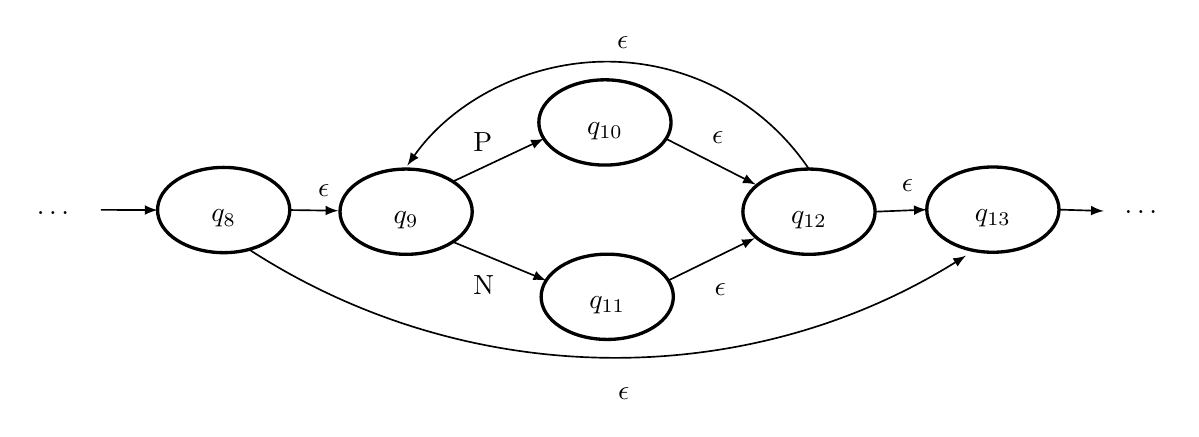
\begin{tikzpicture}
\pgftransformxscale{1.000000}
\pgftransformyscale{-1.000000}
\definecolor{dialinecolor}{rgb}{0.000000, 0.000000, 0.000000}
\pgfsetstrokecolor{dialinecolor}
\definecolor{dialinecolor}{rgb}{1.000000, 1.000000, 1.000000}
\pgfsetfillcolor{dialinecolor}
\definecolor{dialinecolor}{rgb}{1.000000, 1.000000, 1.000000}
\pgfsetfillcolor{dialinecolor}
\pgfpathellipse{\pgfpoint{19.124361\du}{14.988512\du}}{\pgfpoint{0.796261\du}{0\du}}{\pgfpoint{0\du}{0.513512\du}}
\pgfusepath{fill}
\pgfsetlinewidth{0.040000\du}
\pgfsetdash{}{0pt}
\pgfsetdash{}{0pt}
\pgfsetmiterjoin
\definecolor{dialinecolor}{rgb}{0.000000, 0.000000, 0.000000}
\pgfsetstrokecolor{dialinecolor}
\pgfpathellipse{\pgfpoint{19.124361\du}{14.988512\du}}{\pgfpoint{0.796261\du}{0\du}}{\pgfpoint{0\du}{0.513512\du}}
\pgfusepath{stroke}
% setfont left to latex
\definecolor{dialinecolor}{rgb}{0.000000, 0.000000, 0.000000}
\pgfsetstrokecolor{dialinecolor}
\node at (19.124361\du,15.091845\du){$q_{8}$};
\definecolor{dialinecolor}{rgb}{1.000000, 1.000000, 1.000000}
\pgfsetfillcolor{dialinecolor}
\pgfpathellipse{\pgfpoint{28.389361\du}{14.983512\du}}{\pgfpoint{0.796261\du}{0\du}}{\pgfpoint{0\du}{0.513512\du}}
\pgfusepath{fill}
\pgfsetlinewidth{0.040000\du}
\pgfsetdash{}{0pt}
\pgfsetdash{}{0pt}
\pgfsetmiterjoin
\definecolor{dialinecolor}{rgb}{0.000000, 0.000000, 0.000000}
\pgfsetstrokecolor{dialinecolor}
\pgfpathellipse{\pgfpoint{28.389361\du}{14.983512\du}}{\pgfpoint{0.796261\du}{0\du}}{\pgfpoint{0\du}{0.513512\du}}
\pgfusepath{stroke}
% setfont left to latex
\definecolor{dialinecolor}{rgb}{0.000000, 0.000000, 0.000000}
\pgfsetstrokecolor{dialinecolor}
\node at (28.389361\du,15.086845\du){$q_{13}$};
\definecolor{dialinecolor}{rgb}{1.000000, 1.000000, 1.000000}
\pgfsetfillcolor{dialinecolor}
\pgfpathellipse{\pgfpoint{23.716861\du}{13.933512\du}}{\pgfpoint{0.796261\du}{0\du}}{\pgfpoint{0\du}{0.513512\du}}
\pgfusepath{fill}
\pgfsetlinewidth{0.040000\du}
\pgfsetdash{}{0pt}
\pgfsetdash{}{0pt}
\pgfsetmiterjoin
\definecolor{dialinecolor}{rgb}{0.000000, 0.000000, 0.000000}
\pgfsetstrokecolor{dialinecolor}
\pgfpathellipse{\pgfpoint{23.716861\du}{13.933512\du}}{\pgfpoint{0.796261\du}{0\du}}{\pgfpoint{0\du}{0.513512\du}}
\pgfusepath{stroke}
% setfont left to latex
\definecolor{dialinecolor}{rgb}{0.000000, 0.000000, 0.000000}
\pgfsetstrokecolor{dialinecolor}
\node at (23.716861\du,14.036845\du){$q_{10}$};
\definecolor{dialinecolor}{rgb}{1.000000, 1.000000, 1.000000}
\pgfsetfillcolor{dialinecolor}
\pgfpathellipse{\pgfpoint{23.744361\du}{16.033512\du}}{\pgfpoint{0.796261\du}{0\du}}{\pgfpoint{0\du}{0.513512\du}}
\pgfusepath{fill}
\pgfsetlinewidth{0.040000\du}
\pgfsetdash{}{0pt}
\pgfsetdash{}{0pt}
\pgfsetmiterjoin
\definecolor{dialinecolor}{rgb}{0.000000, 0.000000, 0.000000}
\pgfsetstrokecolor{dialinecolor}
\pgfpathellipse{\pgfpoint{23.744361\du}{16.033512\du}}{\pgfpoint{0.796261\du}{0\du}}{\pgfpoint{0\du}{0.513512\du}}
\pgfusepath{stroke}
% setfont left to latex
\definecolor{dialinecolor}{rgb}{0.000000, 0.000000, 0.000000}
\pgfsetstrokecolor{dialinecolor}
\node at (23.744361\du,16.136845\du){$q_{11}$};
\definecolor{dialinecolor}{rgb}{1.000000, 1.000000, 1.000000}
\pgfsetfillcolor{dialinecolor}
\pgfpathellipse{\pgfpoint{21.321861\du}{15.008512\du}}{\pgfpoint{0.796261\du}{0\du}}{\pgfpoint{0\du}{0.513512\du}}
\pgfusepath{fill}
\pgfsetlinewidth{0.040000\du}
\pgfsetdash{}{0pt}
\pgfsetdash{}{0pt}
\pgfsetmiterjoin
\definecolor{dialinecolor}{rgb}{0.000000, 0.000000, 0.000000}
\pgfsetstrokecolor{dialinecolor}
\pgfpathellipse{\pgfpoint{21.321861\du}{15.008512\du}}{\pgfpoint{0.796261\du}{0\du}}{\pgfpoint{0\du}{0.513512\du}}
\pgfusepath{stroke}
% setfont left to latex
\definecolor{dialinecolor}{rgb}{0.000000, 0.000000, 0.000000}
\pgfsetstrokecolor{dialinecolor}
\node at (21.321861\du,15.111845\du){$q_{9}$};
\definecolor{dialinecolor}{rgb}{1.000000, 1.000000, 1.000000}
\pgfsetfillcolor{dialinecolor}
\pgfpathellipse{\pgfpoint{26.174361\du}{15.008512\du}}{\pgfpoint{0.796261\du}{0\du}}{\pgfpoint{0\du}{0.513512\du}}
\pgfusepath{fill}
\pgfsetlinewidth{0.040000\du}
\pgfsetdash{}{0pt}
\pgfsetdash{}{0pt}
\pgfsetmiterjoin
\definecolor{dialinecolor}{rgb}{0.000000, 0.000000, 0.000000}
\pgfsetstrokecolor{dialinecolor}
\pgfpathellipse{\pgfpoint{26.174361\du}{15.008512\du}}{\pgfpoint{0.796261\du}{0\du}}{\pgfpoint{0\du}{0.513512\du}}
\pgfusepath{stroke}
% setfont left to latex
\definecolor{dialinecolor}{rgb}{0.000000, 0.000000, 0.000000}
\pgfsetstrokecolor{dialinecolor}
\node at (26.174361\du,15.111845\du){$q_{12}$};
% setfont left to latex
\definecolor{dialinecolor}{rgb}{0.000000, 0.000000, 0.000000}
\pgfsetstrokecolor{dialinecolor}
\node[anchor=west] at (24.875600\du,14.115000\du){$\epsilon$};
% setfont left to latex
\definecolor{dialinecolor}{rgb}{0.000000, 0.000000, 0.000000}
\pgfsetstrokecolor{dialinecolor}
\node[anchor=west] at (23.731250\du,12.975000\du){$\epsilon$};
% setfont left to latex
\definecolor{dialinecolor}{rgb}{0.000000, 0.000000, 0.000000}
\pgfsetstrokecolor{dialinecolor}
\node[anchor=west] at (20.131250\du,14.750000\du){$\epsilon$};
% setfont left to latex
\definecolor{dialinecolor}{rgb}{0.000000, 0.000000, 0.000000}
\pgfsetstrokecolor{dialinecolor}
\node[anchor=west] at (24.906250\du,15.950000\du){$\epsilon$};
% setfont left to latex
\definecolor{dialinecolor}{rgb}{0.000000, 0.000000, 0.000000}
\pgfsetstrokecolor{dialinecolor}
\node[anchor=west] at (27.163100\du,14.690000\du){$\epsilon$};
% setfont left to latex
\definecolor{dialinecolor}{rgb}{0.000000, 0.000000, 0.000000}
\pgfsetstrokecolor{dialinecolor}
\node[anchor=west] at (23.745600\du,17.200000\du){$\epsilon$};
% setfont left to latex
\definecolor{dialinecolor}{rgb}{0.000000, 0.000000, 0.000000}
\pgfsetstrokecolor{dialinecolor}
\node[anchor=west] at (22\du,14.175000\du){P};
% setfont left to latex
\definecolor{dialinecolor}{rgb}{0.000000, 0.000000, 0.000000}
\pgfsetstrokecolor{dialinecolor}
\node[anchor=west] at (22\du,15.890000\du){N};
% setfont left to latex
\definecolor{dialinecolor}{rgb}{0.000000, 0.000000, 0.000000}
\pgfsetstrokecolor{dialinecolor}
\node[anchor=west] at (16.743800\du,15.025000\du){\dots};
% setfont left to latex
\definecolor{dialinecolor}{rgb}{0.000000, 0.000000, 0.000000}
\pgfsetstrokecolor{dialinecolor}
\node[anchor=west] at (29.846300\du,15.007500\du){\dots};
\pgfsetlinewidth{0.020000\du}
\pgfsetdash{}{0pt}
\pgfsetdash{}{0pt}
\pgfsetbuttcap
{
\definecolor{dialinecolor}{rgb}{0.000000, 0.000000, 0.000000}
\pgfsetfillcolor{dialinecolor}
% was here!!!
\pgfsetarrowsend{latex}
\definecolor{dialinecolor}{rgb}{0.000000, 0.000000, 0.000000}
\pgfsetstrokecolor{dialinecolor}
\draw (19.920623\du,14.988512\du)--(20.505612\du,14.996861\du);
}
\pgfsetlinewidth{0.020000\du}
\pgfsetdash{}{0pt}
\pgfsetdash{}{0pt}
\pgfsetbuttcap
{
\definecolor{dialinecolor}{rgb}{0.000000, 0.000000, 0.000000}
\pgfsetfillcolor{dialinecolor}
% was here!!!
\pgfsetarrowsend{latex}
\definecolor{dialinecolor}{rgb}{0.000000, 0.000000, 0.000000}
\pgfsetstrokecolor{dialinecolor}
\draw (26.970623\du,15.008512\du)--(27.593100\du,14.983512\du);
}
\pgfsetlinewidth{0.020000\du}
\pgfsetdash{}{0pt}
\pgfsetdash{}{0pt}
\pgfsetbuttcap
{
\definecolor{dialinecolor}{rgb}{0.000000, 0.000000, 0.000000}
\pgfsetfillcolor{dialinecolor}
% was here!!!
\pgfsetarrowsend{latex}
\definecolor{dialinecolor}{rgb}{0.000000, 0.000000, 0.000000}
\pgfsetstrokecolor{dialinecolor}
\draw (21.884903\du,14.645404\du)--(22.981212\du,14.130024\du);
}
\pgfsetlinewidth{0.020000\du}
\pgfsetdash{}{0pt}
\pgfsetdash{}{0pt}
\pgfsetbuttcap
{
\definecolor{dialinecolor}{rgb}{0.000000, 0.000000, 0.000000}
\pgfsetfillcolor{dialinecolor}
% was here!!!
\pgfsetarrowsend{latex}
\definecolor{dialinecolor}{rgb}{0.000000, 0.000000, 0.000000}
\pgfsetstrokecolor{dialinecolor}
\draw (21.884903\du,15.371619\du)--(23.008712\du,15.836999\du);
}
\pgfsetlinewidth{0.020000\du}
\pgfsetdash{}{0pt}
\pgfsetdash{}{0pt}
\pgfsetbuttcap
{
\definecolor{dialinecolor}{rgb}{0.000000, 0.000000, 0.000000}
\pgfsetfillcolor{dialinecolor}
% was here!!!
\pgfsetarrowsend{latex}
\definecolor{dialinecolor}{rgb}{0.000000, 0.000000, 0.000000}
\pgfsetstrokecolor{dialinecolor}
\draw (24.452511\du,14.130024\du)--(25.533712\du,14.681652\du);
}
\pgfsetlinewidth{0.020000\du}
\pgfsetdash{}{0pt}
\pgfsetdash{}{0pt}
\pgfsetbuttcap
{
\definecolor{dialinecolor}{rgb}{0.000000, 0.000000, 0.000000}
\pgfsetfillcolor{dialinecolor}
% was here!!!
\pgfsetarrowsend{latex}
\definecolor{dialinecolor}{rgb}{0.000000, 0.000000, 0.000000}
\pgfsetstrokecolor{dialinecolor}
\draw (24.480011\du,15.836999\du)--(25.522020\du,15.327487\du);
}
\pgfsetlinewidth{0.020000\du}
\pgfsetdash{}{0pt}
\pgfsetdash{}{0pt}
\pgfsetbuttcap
{
\definecolor{dialinecolor}{rgb}{0.000000, 0.000000, 0.000000}
\pgfsetfillcolor{dialinecolor}
% was here!!!
\pgfsetarrowsend{latex}
\definecolor{dialinecolor}{rgb}{0.000000, 0.000000, 0.000000}
\pgfsetstrokecolor{dialinecolor}
\pgfpathmoveto{\pgfpoint{26.174378\du}{14.495024\du}}
\pgfpatharc{326}{215}{2.935389\du and 2.935389\du}
\pgfusepath{stroke}
}
\pgfsetlinewidth{0.020000\du}
\pgfsetdash{}{0pt}
\pgfsetdash{}{0pt}
\pgfsetbuttcap
{
\definecolor{dialinecolor}{rgb}{0.000000, 0.000000, 0.000000}
\pgfsetfillcolor{dialinecolor}
% was here!!!
\pgfsetarrowsend{latex}
\definecolor{dialinecolor}{rgb}{0.000000, 0.000000, 0.000000}
\pgfsetstrokecolor{dialinecolor}
\draw (17.643892\du,14.986527\du)--(18.328100\du,14.988512\du);
}
\pgfsetlinewidth{0.020000\du}
\pgfsetdash{}{0pt}
\pgfsetdash{}{0pt}
\pgfsetbuttcap
{
\definecolor{dialinecolor}{rgb}{0.000000, 0.000000, 0.000000}
\pgfsetfillcolor{dialinecolor}
% was here!!!
\pgfsetarrowsend{latex}
\definecolor{dialinecolor}{rgb}{0.000000, 0.000000, 0.000000}
\pgfsetstrokecolor{dialinecolor}
\draw (29.185623\du,14.983512\du)--(29.725000\du,15.000000\du);
}
\pgfsetlinewidth{0.020000\du}
\pgfsetdash{}{0pt}
\pgfsetdash{}{0pt}
\pgfsetbuttcap
{
\definecolor{dialinecolor}{rgb}{0.000000, 0.000000, 0.000000}
\pgfsetfillcolor{dialinecolor}
% was here!!!
\pgfsetarrowsend{latex}
\definecolor{dialinecolor}{rgb}{0.000000, 0.000000, 0.000000}
\pgfsetstrokecolor{dialinecolor}
\pgfpathmoveto{\pgfpoint{19.428607\du}{15.462634\du}}
\pgfpatharc{123}{58}{8.037881\du and 8.037881\du}
\pgfusepath{stroke}
}
\end{tikzpicture}

}
  \caption{Equivalent NFA of direction expression}
\vspace{-2em}
  \label{fig:nfaEx}
\end{figure}
\transtrue
\setcode{standard}


%\begin{figure}[tb!]
%{ \relsize{-1}
%\begin{framed}
%\begin{multicols}{2}
%\begin{itemize}
%\item Annotated Expression: \\
%\\
%{ \relsize{-2.5}
%%\begin{itemize}
%%  \item 
%  $\stackrel{e_1}{(P|N)+}~\stackrel{o_1}{\mathit{O}?}~\stackrel{r}{R}~\stackrel{o_2}{\mathit{O^{\wedge}2}}~\stackrel{e_2}{(P|N|U)+}$
%%\end{itemize}
%}
%\end{itemize}
%\begin{itemize}
%\item User defined semantic \\relations:
%\begin{itemize}
%\item $\langle e_1,e_2,r\rangle$
%\item $\langle r,e_1,o_1\rangle$
%\item $\langle r,e_2,o_2\rangle$
%\end{itemize}
%\end{itemize}
%\columnbreak
%\setcode{utf8}
%\transfalse
%\resizebox{0.9\columnwidth}{!}{
%	\relsize{+1.5} % Graphic for TeX using PGF
% Title: /home/ameen/Desktop/ergraphEx.dia
% Creator: Dia v0.97.1
% CreationDate: Sat Jan 11 03:49:31 2014
% For: ameen
% \usepackage{tikz}
% The following commands are not supported in PSTricks at present
% We define them conditionally, so when they are implemented,
% this pgf file will use them.
\ifx\du\undefined
  \newlength{\du}
\fi
\setlength{\du}{30\unitlength}
\begin{tikzpicture}
\pgftransformxscale{1.000000}
\pgftransformyscale{-1.000000}
\definecolor{dialinecolor}{rgb}{0.000000, 0.000000, 0.000000}
\pgfsetstrokecolor{dialinecolor}
\definecolor{dialinecolor}{rgb}{1.000000, 1.000000, 1.000000}
\pgfsetfillcolor{dialinecolor}
\definecolor{dialinecolor}{rgb}{1.000000, 1.000000, 1.000000}
\pgfsetfillcolor{dialinecolor}
\pgfpathellipse{\pgfpoint{4.324130\du}{10.573360\du}}{\pgfpoint{1.223030\du}{0\du}}{\pgfpoint{0\du}{0.734470\du}}
\pgfusepath{fill}
\pgfsetlinewidth{0.050000\du}
\pgfsetdash{}{0pt}
\pgfsetdash{}{0pt}
\pgfsetmiterjoin
\definecolor{dialinecolor}{rgb}{0.000000, 0.000000, 0.000000}
\pgfsetstrokecolor{dialinecolor}
\pgfpathellipse{\pgfpoint{4.324130\du}{10.573360\du}}{\pgfpoint{1.223030\du}{0\du}}{\pgfpoint{0\du}{0.734470\du}}
\pgfusepath{stroke}
% setfont left to latex
\definecolor{dialinecolor}{rgb}{0.000000, 0.000000, 0.000000}
\pgfsetstrokecolor{dialinecolor}
\node at (4.324130\du,10.465026\du){\RL{دبي مول}};
% setfont left to latex
\definecolor{dialinecolor}{rgb}{0.000000, 0.000000, 0.000000}
\pgfsetstrokecolor{dialinecolor}
\node at (4.324130\du,10.888360\du){Dubai Mall};
\definecolor{dialinecolor}{rgb}{1.000000, 1.000000, 1.000000}
\pgfsetfillcolor{dialinecolor}
\pgfpathellipse{\pgfpoint{6.415976\du}{8.893981\du}}{\pgfpoint{1.395976\du}{0\du}}{\pgfpoint{0\du}{0.720041\du}}
\pgfusepath{fill}
\pgfsetlinewidth{0.050000\du}
\pgfsetdash{}{0pt}
\pgfsetdash{}{0pt}
\pgfsetmiterjoin
\definecolor{dialinecolor}{rgb}{0.000000, 0.000000, 0.000000}
\pgfsetstrokecolor{dialinecolor}
\pgfpathellipse{\pgfpoint{6.415976\du}{8.893981\du}}{\pgfpoint{1.395976\du}{0\du}}{\pgfpoint{0\du}{0.720041\du}}
\pgfusepath{stroke}
% setfont left to latex
\definecolor{dialinecolor}{rgb}{0.000000, 0.000000, 0.000000}
\pgfsetstrokecolor{dialinecolor}
\node at (6.415976\du,8.785647\du){\RL{المبنى}};
% setfont left to latex
\definecolor{dialinecolor}{rgb}{0.000000, 0.000000, 0.000000}
\pgfsetstrokecolor{dialinecolor}
\node at (6.415976\du,9.208981\du){the building};
\definecolor{dialinecolor}{rgb}{1.000000, 1.000000, 1.000000}
\pgfsetfillcolor{dialinecolor}
\pgfpathellipse{\pgfpoint{8.776400\du}{10.616657\du}}{\pgfpoint{0.927400\du}{0\du}}{\pgfpoint{0\du}{0.546667\du}}
\pgfusepath{fill}
\pgfsetlinewidth{0.050000\du}
\pgfsetdash{}{0pt}
\pgfsetdash{}{0pt}
\pgfsetmiterjoin
\definecolor{dialinecolor}{rgb}{0.000000, 0.000000, 0.000000}
\pgfsetstrokecolor{dialinecolor}
\pgfpathellipse{\pgfpoint{8.776400\du}{10.616657\du}}{\pgfpoint{0.927400\du}{0\du}}{\pgfpoint{0\du}{0.546667\du}}
\pgfusepath{stroke}
% setfont left to latex
\definecolor{dialinecolor}{rgb}{0.000000, 0.000000, 0.000000}
\pgfsetstrokecolor{dialinecolor}
\node at (8.776400\du,10.508324\du){\RL{مقربة}};
% setfont left to latex
\definecolor{dialinecolor}{rgb}{0.000000, 0.000000, 0.000000}
\pgfsetstrokecolor{dialinecolor}
\node at (8.776400\du,10.931657\du){near};
\definecolor{dialinecolor}{rgb}{1.000000, 1.000000, 1.000000}
\pgfsetfillcolor{dialinecolor}
\pgfpathellipse{\pgfpoint{4.451892\du}{6.494554\du}}{\pgfpoint{1.451892\du}{0\du}}{\pgfpoint{0\du}{0.787194\du}}
\pgfusepath{fill}
\pgfsetlinewidth{0.050000\du}
\pgfsetdash{}{0pt}
\pgfsetdash{}{0pt}
\pgfsetmiterjoin
\definecolor{dialinecolor}{rgb}{0.000000, 0.000000, 0.000000}
\pgfsetstrokecolor{dialinecolor}
\pgfpathellipse{\pgfpoint{4.451892\du}{6.494554\du}}{\pgfpoint{1.451892\du}{0\du}}{\pgfpoint{0\du}{0.787194\du}}
\pgfusepath{stroke}
% setfont left to latex
\definecolor{dialinecolor}{rgb}{0.000000, 0.000000, 0.000000}
\pgfsetstrokecolor{dialinecolor}
\node at (4.451892\du,6.386221\du){\RL{برج خليفة}};
% setfont left to latex
\definecolor{dialinecolor}{rgb}{0.000000, 0.000000, 0.000000}
\pgfsetstrokecolor{dialinecolor}
\node at (4.451892\du,6.809554\du){Khalifa tower};
\definecolor{dialinecolor}{rgb}{1.000000, 1.000000, 1.000000}
\pgfsetfillcolor{dialinecolor}
\pgfpathellipse{\pgfpoint{6.414368\du}{4.903560\du}}{\pgfpoint{1.590768\du}{0\du}}{\pgfpoint{0\du}{0.722790\du}}
\pgfusepath{fill}
\pgfsetlinewidth{0.050000\du}
\pgfsetdash{}{0pt}
\pgfsetdash{}{0pt}
\pgfsetmiterjoin
\definecolor{dialinecolor}{rgb}{0.000000, 0.000000, 0.000000}
\pgfsetstrokecolor{dialinecolor}
\pgfpathellipse{\pgfpoint{6.414368\du}{4.903560\du}}{\pgfpoint{1.590768\du}{0\du}}{\pgfpoint{0\du}{0.722790\du}}
\pgfusepath{stroke}
% setfont left to latex
\definecolor{dialinecolor}{rgb}{0.000000, 0.000000, 0.000000}
\pgfsetstrokecolor{dialinecolor}
\node at (6.414368\du,4.795227\du){\RL{التقاطع الأول}};
% setfont left to latex
\definecolor{dialinecolor}{rgb}{0.000000, 0.000000, 0.000000}
\pgfsetstrokecolor{dialinecolor}
\node at (6.414368\du,5.218560\du){intersection 1};
\definecolor{dialinecolor}{rgb}{1.000000, 1.000000, 1.000000}
\pgfsetfillcolor{dialinecolor}
\pgfpathellipse{\pgfpoint{8.800968\du}{6.567226\du}}{\pgfpoint{1.083468\du}{0\du}}{\pgfpoint{0\du}{0.584486\du}}
\pgfusepath{fill}
\pgfsetlinewidth{0.050000\du}
\pgfsetdash{}{0pt}
\pgfsetdash{}{0pt}
\pgfsetmiterjoin
\definecolor{dialinecolor}{rgb}{0.000000, 0.000000, 0.000000}
\pgfsetstrokecolor{dialinecolor}
\pgfpathellipse{\pgfpoint{8.800968\du}{6.567226\du}}{\pgfpoint{1.083468\du}{0\du}}{\pgfpoint{0\du}{0.584486\du}}
\pgfusepath{stroke}
% setfont left to latex
\definecolor{dialinecolor}{rgb}{0.000000, 0.000000, 0.000000}
\pgfsetstrokecolor{dialinecolor}
\node at (8.800968\du,6.458893\du){\RL{بالقرب}};
% setfont left to latex
\definecolor{dialinecolor}{rgb}{0.000000, 0.000000, 0.000000}
\pgfsetstrokecolor{dialinecolor}
\node at (8.800968\du,6.882226\du){next to};
% setfont left to latex
\definecolor{dialinecolor}{rgb}{0.000000, 0.000000, 0.000000}
\pgfsetstrokecolor{dialinecolor}
\node at (6.673600\du,10.362490\du){\RL{على}};
% setfont left to latex
\definecolor{dialinecolor}{rgb}{0.000000, 0.000000, 0.000000}
\pgfsetstrokecolor{dialinecolor}
\node at (6.673600\du,10.785823\du){prep};
% setfont left to latex
\definecolor{dialinecolor}{rgb}{0.000000, 0.000000, 0.000000}
\pgfsetstrokecolor{dialinecolor}
\node at (9.098600\du,9.312490\du){\RL{من هذا}};
% setfont left to latex
\definecolor{dialinecolor}{rgb}{0.000000, 0.000000, 0.000000}
\pgfsetstrokecolor{dialinecolor}
\node at (9.098600\du,9.735823\du){from this};
\definecolor{dialinecolor}{rgb}{1.000000, 1.000000, 1.000000}
\pgfsetfillcolor{dialinecolor}
\fill (3.913600\du,8.797490\du)--(3.913600\du,9.615823\du)--(4.733600\du,9.615823\du)--(4.733600\du,8.797490\du)--cycle;
% setfont left to latex
\definecolor{dialinecolor}{rgb}{0.000000, 0.000000, 0.000000}
\pgfsetstrokecolor{dialinecolor}
\node at (4.323600\du,9.112490\du){\RL{مقربة}};
% setfont left to latex
\definecolor{dialinecolor}{rgb}{0.000000, 0.000000, 0.000000}
\pgfsetstrokecolor{dialinecolor}
\node at (4.323600\du,9.535823\du){near};
% setfont left to latex
\definecolor{dialinecolor}{rgb}{0.000000, 0.000000, 0.000000}
\pgfsetstrokecolor{dialinecolor}
\node[anchor=west] at (3.823600\du,8.012500\du){\cci{isSyn}};
% setfont left to latex
\definecolor{dialinecolor}{rgb}{0.000000, 0.000000, 0.000000}
\pgfsetstrokecolor{dialinecolor}
\node at (3.848700\du,4.987490\du){\RL{بالقرب}};
% setfont left to latex
\definecolor{dialinecolor}{rgb}{0.000000, 0.000000, 0.000000}
\pgfsetstrokecolor{dialinecolor}
\node at (3.848700\du,5.410823\du){next to};
% setfont left to latex
\definecolor{dialinecolor}{rgb}{0.000000, 0.000000, 0.000000}
\pgfsetstrokecolor{dialinecolor}
\node at (8.892600\du,5.337490\du){\RL{من}};
% setfont left to latex
\definecolor{dialinecolor}{rgb}{0.000000, 0.000000, 0.000000}
\pgfsetstrokecolor{dialinecolor}
\node at (8.892600\du,5.760823\du){from};
% setfont left to latex
\definecolor{dialinecolor}{rgb}{0.000000, 0.000000, 0.000000}
\pgfsetstrokecolor{dialinecolor}
\node[anchor=west] at (7.103800\du,7.837500\du){};
\pgfsetlinewidth{0.050000\du}
\pgfsetdash{}{0pt}
\pgfsetdash{}{0pt}
\pgfsetbuttcap
{
\definecolor{dialinecolor}{rgb}{0.000000, 0.000000, 0.000000}
\pgfsetfillcolor{dialinecolor}
% was here!!!
\definecolor{dialinecolor}{rgb}{0.000000, 0.000000, 0.000000}
\pgfsetstrokecolor{dialinecolor}
\pgfpathmoveto{\pgfpoint{8.386343\du}{6.027332\du}}
\pgfpatharc{1}{-61}{0.960686\du and 0.960686\du}
\pgfusepath{stroke}
}
\pgfsetlinewidth{0.050000\du}
\pgfsetdash{}{0pt}
\pgfsetdash{}{0pt}
\pgfsetbuttcap
{
\definecolor{dialinecolor}{rgb}{0.000000, 0.000000, 0.000000}
\pgfsetfillcolor{dialinecolor}
% was here!!!
\definecolor{dialinecolor}{rgb}{0.000000, 0.000000, 0.000000}
\pgfsetstrokecolor{dialinecolor}
\pgfpathmoveto{\pgfpoint{4.944705\du}{5.180159\du}}
\pgfpatharc{266}{181}{0.530542\du and 0.530542\du}
\pgfusepath{stroke}
}
\pgfsetlinewidth{0.050000\du}
\pgfsetdash{}{0pt}
\pgfsetdash{}{0pt}
\pgfsetbuttcap
{
\definecolor{dialinecolor}{rgb}{0.000000, 0.000000, 0.000000}
\pgfsetfillcolor{dialinecolor}
% was here!!!
\definecolor{dialinecolor}{rgb}{0.000000, 0.000000, 0.000000}
\pgfsetstrokecolor{dialinecolor}
\pgfpathmoveto{\pgfpoint{5.126282\du}{9.169518\du}}
\pgfpatharc{243}{167}{0.649761\du and 0.649761\du}
\pgfusepath{stroke}
}
\pgfsetlinewidth{0.050000\du}
\pgfsetdash{}{0pt}
\pgfsetdash{}{0pt}
\pgfsetbuttcap
{
\definecolor{dialinecolor}{rgb}{0.000000, 0.000000, 0.000000}
\pgfsetfillcolor{dialinecolor}
% was here!!!
\definecolor{dialinecolor}{rgb}{0.000000, 0.000000, 0.000000}
\pgfsetstrokecolor{dialinecolor}
\pgfpathmoveto{\pgfpoint{8.421500\du}{10.111607\du}}
\pgfpatharc{350}{297}{1.328688\du and 1.328688\du}
\pgfusepath{stroke}
}
\pgfsetlinewidth{0.050000\du}
\pgfsetdash{}{0pt}
\pgfsetdash{}{0pt}
\pgfsetbuttcap
{
\definecolor{dialinecolor}{rgb}{0.000000, 0.000000, 0.000000}
\pgfsetfillcolor{dialinecolor}
% was here!!!
\definecolor{dialinecolor}{rgb}{0.000000, 0.000000, 0.000000}
\pgfsetstrokecolor{dialinecolor}
\pgfpathmoveto{\pgfpoint{5.547041\du}{10.573278\du}}
\pgfpatharc{125}{58}{2.099405\du and 2.099405\du}
\pgfusepath{stroke}
}
\pgfsetlinewidth{0.050000\du}
\pgfsetdash{}{0pt}
\pgfsetdash{}{0pt}
\pgfsetbuttcap
{
\definecolor{dialinecolor}{rgb}{0.000000, 0.000000, 0.000000}
\pgfsetfillcolor{dialinecolor}
% was here!!!
\definecolor{dialinecolor}{rgb}{0.000000, 0.000000, 0.000000}
\pgfsetstrokecolor{dialinecolor}
\pgfpathmoveto{\pgfpoint{4.451867\du}{7.281656\du}}
\pgfpatharc{165}{113}{1.674544\du and 1.674544\du}
\pgfusepath{stroke}
}
% setfont left to latex
\definecolor{dialinecolor}{rgb}{0.000000, 0.000000, 0.000000}
\pgfsetstrokecolor{dialinecolor}
\node[anchor=west] at (6.318700\du,7.975000\du){$e_2$};
% setfont left to latex
\definecolor{dialinecolor}{rgb}{0.000000, 0.000000, 0.000000}
\pgfsetstrokecolor{dialinecolor}
\node[anchor=west] at (4.268700\du,8.825000\du){$r_4$};
% setfont left to latex
\definecolor{dialinecolor}{rgb}{0.000000, 0.000000, 0.000000}
\pgfsetstrokecolor{dialinecolor}
\node[anchor=west] at (4.198700\du,11.665000\du){$e_1$};
% setfont left to latex
\definecolor{dialinecolor}{rgb}{0.000000, 0.000000, 0.000000}
\pgfsetstrokecolor{dialinecolor}
\node[anchor=west] at (8.868700\du,11.525000\du){$r_4$};
% setfont left to latex
\definecolor{dialinecolor}{rgb}{0.000000, 0.000000, 0.000000}
\pgfsetstrokecolor{dialinecolor}
\node[anchor=west] at (8.881200\du,8.915000\du){$o_2$};
% setfont left to latex
\definecolor{dialinecolor}{rgb}{0.000000, 0.000000, 0.000000}
\pgfsetstrokecolor{dialinecolor}
\node[anchor=west] at (6.533700\du,11.315000\du){$o_1$};
% setfont left to latex
\definecolor{dialinecolor}{rgb}{0.000000, 0.000000, 0.000000}
\pgfsetstrokecolor{dialinecolor}
\node[anchor=west] at (3.046200\du,7.390000\du){$e_1$};
% setfont left to latex
\definecolor{dialinecolor}{rgb}{0.000000, 0.000000, 0.000000}
\pgfsetstrokecolor{dialinecolor}
\node[anchor=west] at (6.298700\du,3.940000\du){$e_2$};
% setfont left to latex
\definecolor{dialinecolor}{rgb}{0.000000, 0.000000, 0.000000}
\pgfsetstrokecolor{dialinecolor}
\node[anchor=west] at (8.753700\du,5.015000\du){$o_2$};
% setfont left to latex
\definecolor{dialinecolor}{rgb}{0.000000, 0.000000, 0.000000}
\pgfsetstrokecolor{dialinecolor}
\node[anchor=west] at (3.781200\du,4.590000\du){$r_1$};
% setfont left to latex
\definecolor{dialinecolor}{rgb}{0.000000, 0.000000, 0.000000}
\pgfsetstrokecolor{dialinecolor}
\node[anchor=west] at (8.708700\du,7.490000\du){$r_1$};
\end{tikzpicture}

%}
%\transtrue
%\setcode{standard}
%\end{multicols}
%\end{framed}
%}
%\caption{User-defined semantic relation example}
%\label{fig:srEx}
%\end{figure}

\framework computes the relational entities in a user defined 
relation $R=\ldbrack \langle e_1,e_2,r\rangle \rdbrack
\subseteq \ldbrack e_1 \rdbrack \times \ldbrack e_2 \rdbrack \times \ldbrack r \rdbrack$ 
to be the elements of $\ldbrack e_1 \rdbrack \times \ldbrack e_2 \rdbrack \times \ldbrack r \rdbrack$
with the smallest nonzero positive distance between the source and the destination
where the distance is the number of words between the matches. 

%\framework supports the following configurations for the subexpressions of $e_i$ and $e_j$:
%\begin{itemize}
%\item $\left\vert{e_i}\right\vert=1\wedge\left\vert{e_j}\right\vert=1$: Relate $e_i$ match to $e_j$ match with edge labelled by $r$.
%\item $i=j\wedge\left\vert{e_i}\right\vert>1$: Relate sequences of $e_i$ matches with edges labelled by $r$.
%\item $i\neq j\wedge\left\vert{e_i}\right\vert>1\wedge\left\vert{e_j}\right\vert=1$: Relate each $e_i$ match to the single $e_j$ match with an edge labelled by $r$. The reverse applies for $\left\vert{e_i}\right\vert=1\wedge\left\vert{e_j}\right\vert>1$.
%\item $i\neq j\wedge\left\vert{e_i}\right\vert>1\wedge\left\vert{e_j}\right\vert>1$: Relate each $e_i$ match to each $e_j$ match with an edge labelled by $r$.
%\end{itemize}
%
In Figure~\ref{fig:motiv}(b), \framework names the subexpressions 
$(P|N)+$, $(P|N|U)+$, $O?$, $O\wedge 2$, and $R$, 
as $e_1, e_2, o_1, o_2,$ and $r$, respectively. 
The user defines the semantic relations
$\langle e_1, e_2, r\rangle$, 
$\langle r, e_1, o_1\rangle$, and 
$\langle r,e_2,o_2\rangle$.

The matches of $e_1,~e_2,~o_1,~o_2,$ and $r$ from the second match tree 
of Figure~\ref{fig:motiv}(b) are \RL{dby mwl}(Dubai Mall), 
\RL{Almbn_A}(the building), \RL{`l_A}(prep), \RL{mn h_dA}(from this), 
and \RL{mqrbT}(near), respectively. 
\framework~constructs the semantic relation matches and builds the lower part of the 
entity-relation graph shown in Figure~\ref{fig:intromotiv}.

Similarly, for the  
first match \RL{brj _hlyfT bAlqrb mn AltqA.t` Al-'-wl},
the matches of $e_1,~e_2,~o_2,$ and $r$ are 
\RL{brj _hlyfT}(Khalifa tower), \RL{AltqA.t` Al-'-wl}(intersection 1), 
\RL{mn}(from), and \RL{bAlqrb}(next to), respectively. 
\framework~doesn't construct the relation $\langle r, e_1, o_1\rangle$ 
since $o_1$ has no match. 
Therefore, we get the upper part of the entity-relation graph shown 
in Figure~\ref{fig:intromotiv}.

After computing the relational entities, 
\framework~computes a cross-reference relation between the extracted entities
using a second order synonymy feature ($Syn^2$).
The \cci{isA} edge in the 
graph of Figure~\ref{fig:intromotiv} shows the cross-reference relation 
between \RL{brj _hlyfT}(Khalifa tower) from the first match 
with \RL{Almbn_A}(the building) from the second match. 
